% Отчёт: регрессионная корректировка Лина с HC2 (VarWar R&D v3)
% Сборка: docs/reports/lin_hc2/build.sh  (XeLaTeX через tectonic)
\documentclass[11pt,a4paper]{article}

\usepackage{fontspec}
\usepackage{polyglossia}
\setdefaultlanguage{russian}
\setotherlanguage{english}
\setmainfont{cmunrm}[Extension=.otf,BoldFont=cmunbx,ItalicFont=cmunti,BoldItalicFont=cmunbi]
\setsansfont{cmunss}[Extension=.otf,BoldFont=cmunsx,ItalicFont=cmunsi,BoldItalicFont=cmunso]
\setmonofont{cmuntt}[Extension=.otf,BoldFont=cmuntb,ItalicFont=cmunit,BoldItalicFont=cmuntx]
\newfontfamily\cyrillicfont{cmunrm}[Extension=.otf,BoldFont=cmunbx,ItalicFont=cmunti,BoldItalicFont=cmunbi]
\newfontfamily\cyrillicfontsf{cmunss}[Extension=.otf,BoldFont=cmunsx,ItalicFont=cmunsi,BoldItalicFont=cmunso]
\newfontfamily\cyrillicfonttt{cmuntt}[Extension=.otf,BoldFont=cmuntb,ItalicFont=cmunit,BoldItalicFont=cmuntx]

\usepackage{amsmath,amssymb,amsthm,mathtools,bm}
\usepackage[round,authoryear]{natbib}
\usepackage{booktabs,array,tabularx,multirow}
\usepackage{graphicx}
\usepackage[margin=2.3cm]{geometry}
\usepackage{enumitem}
\setlist{nosep,leftmargin=*}
\usepackage{xcolor}
\definecolor{linkblue}{HTML}{1F5FAE}
\usepackage[colorlinks=true,linkcolor=linkblue,citecolor=linkblue,urlcolor=linkblue]{hyperref}
\usepackage{caption}
\captionsetup{font=small,labelfont=bf,labelsep=period}
\usepackage{titlesec}
\titleformat{\section}{\large\bfseries}{\thesection.}{0.5em}{}
\titleformat{\subsection}{\normalsize\bfseries}{\thesubsection.}{0.5em}{}

\theoremstyle{plain}
\newtheorem{proposition}{Утверждение}
\newtheorem{theorem}{Теорема}
\theoremstyle{definition}
\newtheorem{definition}{Определение}
\theoremstyle{remark}
\newtheorem{remark}{Замечание}

\newcommand{\E}{\mathbb{E}}
\newcommand{\Var}{\operatorname{Var}}
\newcommand{\Cov}{\operatorname{Cov}}
\newcommand{\SE}{\operatorname{SE}}
\newcommand{\T}{^{\top}}
\newcommand{\codeus}{\textunderscore\allowbreak}
\newcommand{\code}[1]{{\small\ttfamily\let\_\codeus #1}}

\title{\textbf{Регрессионная корректировка Лина с робастной дисперсией HC2\\ для анализа A/B-тестов}\\[0.4em]
\large Теория, реализация в VarWar и численная проверка}
\author{VarWar R\&D, ветка \code{rerun/v3.1}}
\date{20 октября 2026}

\setlength{\emergencystretch}{3em}
\begin{document}
\maketitle

\begin{abstract}
\noindent
Отчёт описывает пайплайн подведения итогов A/B-теста, который по результатам
ревизии R\&D VarWar~v3 выглядит наиболее перспективным: полная рандомизация,
без преобразования метрики, \emph{регрессионная корректировка Лина}
(OLS с центрированными предэкспериментальными ковариатами и их взаимодействиями
с воздействием) и робастная ковариационная матрица \emph{HC2} с $t$-квантилем.
Мы выводим эстиматор и его закрытую форму, объясняем, почему он
асимптотически не хуже разности средних и ANCOVA/CUPED при любом соотношении групп
(ответ Лина на критику Фридмана), и подробно разбираем статистический вывод:
консервативность HC2 для выборочного эффекта (SATE), поправку для популяционного
эффекта (PATE), поведение при малых выборках, мощность и MDE. Численная часть
опирается на результаты стенда VarWar~v3 (1000 реализаций в подтверждающем мире и
200 реализаций в 24 мирах) и на независимые Monte-Carlo проверки. В подтверждающем
мире ($n=200$, $R^2=0.4$) Lin+HC2 сохраняет номинальный размер теста
($\widehat{\text{FPR}}=0.048$) и покрытие ($0.95$), снижая MSE на 37\% относительно
разности средних. Полный пересчёт по всем мирам подготовлен и выполняется отдельно.
\end{abstract}

\tableofcontents
\bigskip

%=====================================================================
\section{Контекст и выбор пайплайна}
%=====================================================================

VarWar сравнивает \emph{полные процедуры} анализа рандомизированного эксперимента:
\[
\text{FeatureAdapter}\to\text{Structure}\to\text{Assignment}\to
\text{TargetTransformer}\to\text{AnalysisMethod},
\]
где \code{AnalysisMethod} --- согласованная пара «точечная оценка + статистический вывод».
Каноническим идентификатором рассматриваемого пайплайна является
\begin{center}\footnotesize\ttfamily
adapt.identity\_\_structure.none\_\_assign.complete\_randomization\_\_\\
target.identity\_\_analysis.lin\_regression\_\_hc2
\end{center}

\paragraph{Почему именно он.} Ревизия стенда (46 подтверждённых находок, см.
\code{docs/review/v3\_review\_design.md}) показала следующее.
\begin{enumerate}
  \item Для пайплайнов с преобразованием метрики (CUPED, CUPAC) в v3
        стандартная ошибка вычислялась по \emph{исходной}, а не по преобразованной метрике,
        поэтому их размер теста, покрытие и мощность в опубликованных таблицах некорректны
        (исправлено в ветке \code{rerun/v3.1}, требуется пересчёт).
        Оценки Лина и ML-RATE используют \emph{собственную} (нативную) SE и этой ошибкой не затронуты.
  \item Среди процедур с корректным выводом Lin+HC2 имеет наименьший RMSE в
        подтверждающем мире и в большинстве миров screening, при этом он строго
        обобщает канонический бейзлайн стенда: без ковариат HC2 совпадает с Welch (Утверждение~\ref{prop:welch}).
  \item ML-RATE с линейным ridge-прогнозом в v3 численно неотличим от Лина:
        прогноз строится по тем же признакам. Нелинейный вариант (градиентный бустинг)
        добавлен в ветке \code{rerun/v3.1} и будет сравниваться при пересчёте.
\end{enumerate}

%=====================================================================
\section{Постановка задачи}
%=====================================================================

Рассмотрим $n$ единиц рандомизации (например, клиентов). У единицы $i$ есть
потенциальные исходы $Y_i(1)$, $Y_i(0)$ и вектор ковариат $X_i\in\mathbb R^K$,
\emph{измеренных до назначения воздействия} (предпериод). Индикатор воздействия
$T_i\in\{0,1\}$; наблюдаем $Y_i=T_iY_i(1)+(1-T_i)Y_i(0)$ (SUTVA).

\begin{definition}[Полная рандомизация]
Ровно $n_1$ из $n$ единиц случайно выбираются в тестовую группу, все
$\binom{n}{n_1}$ назначений равновероятны; $p=n_1/n$, $n_0=n-n_1$.
\end{definition}

Целевые величины (estimand):
\[
\tau_{\text{SATE}}=\frac1n\sum_{i=1}^n\bigl(Y_i(1)-Y_i(0)\bigr),\qquad
\tau_{\text{PATE}}=\E\bigl[Y(1)-Y(0)\bigr].
\]
SATE --- эффект в экспериментальной когорте (основная дорожка стенда, \code{sample\_ate}),
PATE --- эффект в популяции, из которой когорта является случайной выборкой.
В конечно-популяционной (дизайновой) постановке случайность возникает
\emph{только} из назначения; в суперпопуляционной --- ещё и из выборки единиц.

Требование «ковариаты до воздействия» принципиально: если $X_i$ может зависеть от
$T_i$, корректировка вычитает часть эффекта, и оценка смещается
(в старом прототипе это давало смещение около 40\%).

%=====================================================================
\section{Эстиматор}
%=====================================================================

\subsection{Модель и закрытая форма}

Пусть $\bar X=n^{-1}\sum_i X_i$ и $\tilde X_i=X_i-\bar X$ --- ковариаты,
центрированные по \emph{всей} выборке. Оценка Лина \citep{lin2013} --- коэффициент
при $T_i$ в OLS-регрессии
\begin{equation}\label{eq:lin}
Y_i=\alpha+\tau T_i+\tilde X_i\T\beta+T_i\,\tilde X_i\T\gamma+e_i .
\end{equation}
В матричной записи $W_i=(1,T_i,\tilde X_i\T,T_i\tilde X_i\T)\T\in\mathbb R^{2K+2}$,
$\hat\theta=(W\T W)^{-1}W\T Y$, $\hat\tau_L=\hat\theta_T$.

\begin{proposition}[Закрытая форма]\label{prop:closed}
Пусть $\hat\beta_1,\hat\beta_0$ --- OLS-наклоны регрессии $Y$ на $X$ (с константой)
отдельно в тестовой и контрольной группах. Тогда
\begin{equation}\label{eq:closed}
\hat\tau_L=\Bigl[\bar Y_1-(\bar X_1-\bar X)\T\hat\beta_1\Bigr]-\Bigl[\bar Y_0-(\bar X_0-\bar X)\T\hat\beta_0\Bigr]
=\frac1n\sum_{i=1}^n\bigl(\hat\mu_1(X_i)-\hat\mu_0(X_i)\bigr),
\end{equation}
где $\hat\mu_t(x)$ --- линейный прогноз, построенный по группе $t$.
\end{proposition}

\begin{proof}[Набросок]
Регрессия \eqref{eq:lin} насыщена по группам: у каждой группы свои свободный член и
наклоны, поэтому её подгонка совпадает с двумя отдельными регрессиями.
В контроле $\hat\alpha+\tilde x\T\hat\beta=\hat\mu_0(x)$, в тесте
$\hat\alpha+\hat\tau+\tilde x\T(\hat\beta+\hat\gamma)=\hat\mu_1(x)$.
При $x=\bar X$ получаем $\hat\tau=\hat\mu_1(\bar X)-\hat\mu_0(\bar X)$,
а по линейности $\hat\mu_t(\bar X)=n^{-1}\sum_i\hat\mu_t(X_i)$.
Наконец, $\hat\mu_t(\bar X)=\bar Y_t+(\bar X-\bar X_t)\T\hat\beta_t$, так как OLS-прямая проходит через $(\bar X_t,\bar Y_t)$.
\end{proof}

Формула \eqref{eq:closed} даёт три полезные интерпретации:
\begin{itemize}
  \item \emph{скорректированные средние}: среднее каждой группы сдвигается к общему
        среднему ковариат по своему наклону;
  \item \emph{импутация}: для каждой единицы оба потенциальных исхода предсказываются
        групповыми моделями, и разность усредняется по всей когорте;
  \item \emph{частные случаи}: при $K=0$ это разность средних
        $\hat\tau_{\text{DM}}=\bar Y_1-\bar Y_0$; при принудительно общем наклоне
        $\hat\beta_1=\hat\beta_0$ это ANCOVA; CUPED с одной ковариатой и общим $\theta$ ---
        тот же класс.
\end{itemize}
Используя $\bar X_1-\bar X=(1-p)(\bar X_1-\bar X_0)$ и $\bar X_0-\bar X=-p(\bar X_1-\bar X_0)$,
\begin{equation}\label{eq:theta-form}
\hat\tau_L=\hat\tau_{\text{DM}}-\bigl[(1-p)\hat\beta_1+p\,\hat\beta_0\bigr]\T(\bar X_1-\bar X_0).
\end{equation}

\subsection{Класс линейно скорректированных оценок и оптимальный коэффициент}

Рассмотрим класс
$\hat\tau(\theta)=\hat\tau_{\text{DM}}-\theta\T(\bar X_1-\bar X_0)$ с фиксированным
$\theta\in\mathbb R^K$. При полной рандомизации любая оценка класса несмещена для SATE,
а её асимптотическая дисперсия
\begin{equation}\label{eq:var-theta}
n\Var\hat\tau(\theta)\;\to\;\frac{\Var\bigl(Y(1)-\theta\T X\bigr)}{p}
+\frac{\Var\bigl(Y(0)-\theta\T X\bigr)}{1-p}-\Var\bigl(\tau_i\bigr)
\end{equation}
(последнее слагаемое не зависит от $\theta$). Минимизация по $\theta$ даёт
\begin{equation}\label{eq:theta-star}
\theta^*=(1-p)\,\beta_1+p\,\beta_0,\qquad \beta_t=\Sigma_X^{-1}\Cov\bigl(X,Y(t)\bigr).
\end{equation}
Сравнивая с \eqref{eq:theta-form}, видим, что оценка Лина асимптотически использует
именно $\theta^*$: она \emph{оптимальна в классе}.

\subsection{Критика Фридмана и ответ Лина}

ANCOVA (регрессия без взаимодействий) и CUPED с $\theta$, оценённым по всей
выборке, сходятся к коэффициенту с \emph{перепутанными весами}:
$\theta_{\text{pool}}=p\,\beta_1+(1-p)\,\beta_0$ \citep{freedman2008}. Подставляя
в \eqref{eq:var-theta}, получаем потерю эффективности
\begin{equation}\label{eq:freedman-loss}
n\bigl[\Var\hat\tau_{\text{ANCOVA}}-\Var\hat\tau_L\bigr]\;\to\;
\frac{(1-2p)^2}{p(1-p)}\,(\beta_1-\beta_0)\T\Sigma_X(\beta_1-\beta_0)\;\ge 0 .
\end{equation}
Потеря исчезает при $p=1/2$ или при одинаковых наклонах. При неравном сплите и
гетерогенных наклонах ANCOVA/CUPED может оказаться \emph{хуже разности средних};
Лин --- никогда (асимптотически). Пример из раздела~\ref{sec:numeric}: при $p=0.2$,
$\beta_0=1$, $\beta_1=0$ дисперсия ANCOVA и CUPED составляет $1.42$ и $1.40$ от
дисперсии разности средних, а дисперсия Лина --- $0.95$.

Фридман также указывал, что классическая OLS-дисперсия ANCOVA может быть
несостоятельной. Лин показал, что обе претензии снимаются одновременно: нужны
\emph{взаимодействия} и \emph{робастная (сэндвич) дисперсия}.

%=====================================================================
\section{Статистический вывод}
%=====================================================================

\subsection{Асимптотическое распределение}

Обозначим через $e_i(t)=Y_i(t)-\bar Y(t)-(X_i-\bar X)\T\beta_t$ остатки
конечно-популяционных проекций потенциальных исходов на ковариаты,
$S^2_{e(t)}$ --- их дисперсии, $S^2_{e(1)-e(0)}$ --- дисперсия разности.

\begin{theorem}[\citealp{lin2013}; \citealp{lidingclt2017}]\label{thm:clt}
При полной рандомизации, фиксированном $K$, $p\to p_\infty\in(0,1)$ и стандартных
условиях на моменты и рычаги ($\max_i h_{ii}\to0$)
\[
\sqrt n\,(\hat\tau_L-\tau_{\text{SATE}})\;\xrightarrow{d}\;
\mathcal N\!\Bigl(0,\;\sigma^2_L\Bigr),\qquad
\sigma^2_L=\frac{S^2_{e(1)}}{p}+\frac{S^2_{e(0)}}{1-p}-S^2_{e(1)-e(0)} .
\]
Кроме того, $\sigma^2_L\le\sigma^2_{\text{DM}}$ и $\sigma^2_L\le\sigma^2_{\text{ANCOVA}}$.
\end{theorem}

Результат \emph{агностичен}: линейная модель не обязана быть верной. Неверная
спецификация лишь уменьшает выигрыш в точности, но не ломает несмещённость
(смещение имеет порядок $O(1/n)$) и не ломает вывод.

\subsection{Робастная дисперсия HC2}

Пусть $\hat e_i$ --- остатки регрессии \eqref{eq:lin}, $h_{ii}=W_i\T(W\T W)^{-1}W_i$ --- рычаги.
Семейство сэндвич-оценок:
\begin{equation}\label{eq:hc}
\hat V_{\text{HC}m}=(W\T W)^{-1}\Bigl(\sum_{i=1}^n\frac{\hat e_i^2}{(1-h_{ii})^{m}}\,W_iW_i\T\Bigr)(W\T W)^{-1},
\qquad m=0,1,2 \;\;(\text{HC0, HC2, HC3}),
\end{equation}
$\widehat{\SE}=\sqrt{[\hat V]_{TT}}$ \citep{whitehc, mackinnonwhite1985}.

\begin{proposition}[HC2 без ковариат = Welch]\label{prop:welch}
При $K=0$
$[\hat V_{\text{HC2}}]_{TT}=s_1^2/n_1+s_0^2/n_0$, где $s_t^2$ --- несмещённые
выборочные дисперсии в группах.
\end{proposition}
\begin{proof}[Набросок]
При $W_i=(1,T_i)$ рычаг $h_{ii}=1/n_{T_i}$, остаток --- отклонение от группового среднего.
Тогда $\sum_{i:T_i=t}\hat e_i^2/(1-1/n_t)=n_t s_t^2$, и сэндвич для $\tau$ равен
$\sum_t n_t s_t^2/n_t^2$.
\end{proof}

С ковариатами HC2 асимптотически эквивалентна нейманновской оценке на остатках:
\[
[\hat V_{\text{HC2}}]_{TT}=\frac{\hat s^2_{e,1}}{n_1}+\frac{\hat s^2_{e,0}}{n_0}+o_p(n^{-1}).
\]
Её математическое ожидание не учитывает отрицательный член $-S^2_{e(1)-e(0)}/n$
теоремы~\ref{thm:clt}, поэтому
\begin{equation}\label{eq:conservative}
\E\,[\hat V_{\text{HC2}}]_{TT}-\Var(\hat\tau_L)\approx\frac{S^2_{e(1)-e(0)}}{n}\ge0 :
\end{equation}
\emph{для SATE оценка HC2 консервативна}. Консервативность исчезает, если
эффект линеен по $X$ (остатки $e(1)$ и $e(0)$ совпадают), и это неустранимо:
индивидуальные эффекты не наблюдаются.

\subsection{Популяционный эффект и поправка}

Если цель --- PATE, а когорта является случайной выборкой из популяции, к дисперсии
добавляется неопределённость $\bar X$ как оценки $\E X$:
\begin{equation}\label{eq:pate}
\widehat\Var_{\text{PATE}}(\hat\tau_L)=[\hat V_{\text{HC2}}]_{TT}+\frac1n\,\hat\gamma\T\hat\Sigma_X\hat\gamma,
\qquad\hat\gamma=\hat\beta_1-\hat\beta_0 .
\end{equation}
Поправка ненулевая только при гетерогенных наклонах. Без неё интервал для PATE
антиконсервативен: в нашей проверке покрытие PATE было $0.931$ при $p=0.2$ и $0.920$ при
$p=0.5$, с поправкой --- $0.953$ и $0.951$ (табл.~\ref{tab:freedman}).
Если веса целевой популяции отличаются от когорты (сдвиг популяции),
оценка переносится как $\hat\tau_L+(\mu^*-\bar X)\T\hat\gamma$ с соответствующей
дельта-методной дисперсией. Это отдельная дорожка \code{population\_ate}:
её нельзя ранжировать вместе с SATE.

\subsection{Доверительный интервал, p-value и малые выборки}

Интервал и двусторонний p-value:
\[
\hat\tau_L\pm t_{1-\alpha/2,\;\nu}\,\widehat{\SE},\qquad
p=2\Bigl(1-F_{t_\nu}\bigl(|\hat\tau_L|/\widehat{\SE}\bigr)\Bigr),\qquad \nu=n-(2K+2).
\]
Асимптотически квантиль нормальный; $t_\nu$ --- консервативная поправка на конечное $n$.
Эквивалентно, тест отвергает $H_0:\tau=0$ ровно тогда, когда $0\notin$ CI.

При малом числе наблюдений на параметр HC2 занижает дисперсию, так как остатки
OLS «прилипают» к данным. Наша проверка (рис.~\ref{fig:smalln}, сплит 30/70, $K=5$,
гетероскедастичность) даёт следующее:
\begin{itemize}
  \item при $n=40$ (около 12 наблюдений в тестовой группе на 12 параметров)
        покрытие HC2 равно $0.928$, HC3 --- $0.984$ (перестраховка);
  \item при $n\ge200$ оба варианта близки к $0.95$.
\end{itemize}
Практическое правило: держать $K\ll\min(n_1,n_0)$ (ориентир --- не более $n_{\min}/20$);
при малых $n$ использовать HC3 или поправку числа степеней свободы
Белла--Маккаффри \citep{bellmccaffrey2002, imbenskolesar2016}.

\subsection{Мощность и минимальный детектируемый эффект}

Пусть $R^2$ --- доля дисперсии $Y$, объяснённая ковариатами внутри группы
(вне выборки обучения). Тогда приближённо
\[
\SE(\hat\tau_L)\approx\sigma_Y\sqrt{1-R^2}\,\sqrt{\frac1{n_1}+\frac1{n_0}}\;\Bigl(1+O\bigl(\tfrac{K}{n}\bigr)\Bigr),
\qquad
\text{MDE}_{1-\beta}=\bigl(t_{1-\alpha/2,\nu}+t_{1-\beta,\nu}\bigr)\,\SE .
\]
Необходимый объём выборки уменьшается в $1/(1-R^2)$ раз; экономия равна $R^2$.
Для дизайна эксперимента $R^2$ нужно брать из исторических данных вне выборки:
in-sample $R^2$ оптимистичен. В подтверждающем мире VarWar ($R^2=0.4$, $n=200$, $K=5$)
теоретическое снижение дисперсии составляет $1-0.6\,(1+10/200)=0.37$, наблюдаемое ---
$0.367$ (табл.~\ref{tab:confirm}).

%=====================================================================
\section{Обобщение: прогноз машинного обучения как ковариата}
%=====================================================================

Если сигнал нелинеен или признаков много, ковариаты сворачиваются в один прогноз
$\hat g(X)$ исхода (идея CUPAC и ML-RATE, \citealp{guo2021mlrate}), который подаётся в
\eqref{eq:lin} вместо $X$ (или вместе с лагом самой метрики):
\[
Y_i=\alpha+\tau T_i+\beta\bigl(\hat g_i-\bar{\hat g}\bigr)+\delta\,T_i\bigl(\hat g_i-\bar{\hat g}\bigr)+e_i .
\]
Здесь критично, \emph{на каких данных обучена} модель $\hat g$.
\begin{itemize}
  \item \textbf{Только предпериод} (temporal CUPAC, «lag2$\to$lag1»): $\hat g_i$ ---
        фиксированная функция данных до воздействия, и теория Лина применяется без изменений.
  \item \textbf{Cross-fitting} (ML-RATE): выборка делится на $K_f$ фолдов, и
        $\hat g_i=\hat g^{(-k(i))}(X_i)$ обучается без фолда единицы $i$ и без $T$.
        Условно на остальные фолды $\hat g_i$ --- функция только $X_i$, поэтому
        валидность сохраняется при любом качестве модели \citep{chernozhukov2018dml, guo2021mlrate}.
  \item \textbf{In-sample} (модель обучена на тех же исходах эксперимента и применена
        к тем же строкам) \emph{запрещено}. Для линейного сглаживателя $\hat g=SY$
        получаем $\E\hat\tau\approx\tau\,(1-\operatorname{tr}S/n)$: часть эффекта «съедается»,
        а снижение дисперсии завышается. Именно эта ошибка была в прототипах на
        реальных данных.
\end{itemize}
Включать лаг самой метрики в число ковариат полезно: тогда Лин с прогнозом
асимптотически не хуже CUPED по этому лагу, даже если модель $\hat g$ деградировала
из-за дрейфа.

%=====================================================================
\section{Реализация в VarWar}
%=====================================================================

\begin{table}[h]
\centering\small
\caption{Где реализован пайплайн.}\label{tab:impl}
\begin{tabularx}{\textwidth}{@{}lX@{}}
\toprule
Компонент & Реализация \\
\midrule
Регистрация & \code{analysis\_registry.py}: метод \code{lin\_regression\_\_hc2} = \code{RegressionAdjustmentEstimator} с \code{covariance\_type="HC2"}; estimand \code{sample\_ate}; нативный вывод \\
Точка и SE & \code{estimators.py: RegressionAdjustmentEstimator.estimate} --- центрирование, матрица $W$, OLS через \code{lstsq} \\
Ковариация & \code{estimators.py: \_robust\_covariance} --- \code{pinv}$(W\T W)$, $h_{ii}$ через \code{einsum}, веса $\hat e_i^2/\max(1-h_{ii},10^{-12})$ \\
CI и p-value & \code{estimators.py: \_build\_result} --- $t_\nu$, $\nu=n-\dim W$ \\
Ковариаты в гонке & \code{rnd\_runner.py: \_spec} --- \code{pre\_target\_lag1, x1, x2, x3, x4} ($K=5$, $\dim W=12$) \\
\bottomrule
\end{tabularx}
\end{table}

Численная сверка: оценка и SE (HC2 и HC3) совпадают со \code{statsmodels} до $10^{-15}$;
без ковариат SE совпадает с Welch. Изменения ветки \code{rerun/v3.1}, затрагивающие этот пайплайн:
\begin{itemize}
  \item центрирование ковариат выполняется по строкам, реально участвующим в
        регрессии (раньше --- по всем строкам до фильтра пропусков);
  \item в диагностику выводится ранг матрицы плана (коллинеарность больше не
        маскируется \code{pinv});
  \item миры с гетерогенным эффектом получили настоящую нулевую гипотезу для SATE
        (раньше «H0» в мире сдвига популяции имела SATE$\,=0.285$, и FPR$\,=1$ был мощностью);
  \item правила вердиктов учитывают Monte-Carlo-ошибку; seed не зависят от
        шардирования; нелинейный ML-RATE добавлен как конкурент.
\end{itemize}
Там же добавлены опции, относящиеся к выводу: вариант \code{lin\_regression\_\_hc2\_pate}
с поправкой \eqref{eq:pate} (только для дорожки \code{population\_ate}; предполагает, что
когорта --- iid-выборка из целевой популяции) и необязательные степени свободы
Белла--Маккаффри для HC2 (по умолчанию выключены).
Известное ограничение: категориальные ковариаты (\code{region}, \code{device}) в гонке
не используются.

%=====================================================================
\section{Численная проверка}\label{sec:numeric}
%=====================================================================

\subsection{Подтверждающий мир стенда v3}

Мир \code{gaussian\_r2\_04\_n200}: $n=200$, сплит 50/50, $R^2=0.4$, 1000 реализаций,
общие случайные числа для всех процедур (табл.~\ref{tab:confirm}). FPR оценён под $H_0$,
остальные метрики --- при эффекте $0.2\sigma$; в квадратных скобках --- 95\% интервал Уилсона.

\begin{table}[h]
\centering\small
\caption{Подтверждение (VarWar v3, $R=1000$). Строки CUPED/CUPAC не приводятся: их SE в v3 была вычислена неверно.}\label{tab:confirm}
\footnotesize\setlength{\tabcolsep}{3.5pt}
\begin{tabular}{@{}lccccccc@{}}
\toprule
Метод & FPR & Покрытие & Смещение & SD & $\overline{\SE}$ & SE/SD & RMSE \\
\midrule
Welch (разность средних) & 0.047 {\scriptsize[0.036; 0.062]} & 0.955 & $-0.0035$ & 0.135 & 0.141 & 1.04 & 0.135 \\
\textbf{Лин + HC2} & \textbf{0.048} {\scriptsize[0.036; 0.063]} & \textbf{0.954} & $-0.0044$ & \textbf{0.108} & 0.111 & 1.03 & \textbf{0.108} \\
ML-RATE (ridge, cross-fit) + HC2 & 0.047 {\scriptsize[0.036; 0.062]} & 0.955 & $-0.0024$ & 0.109 & 0.112 & 1.03 & 0.109 \\
\bottomrule
\end{tabular}

\smallskip
\begin{tabular}{@{}lccc@{}}
\toprule
Метод & Снижение дисперсии vs Welch & Мощность при $0.2\sigma$ & Медиана времени, мс \\
\midrule
Welch & --- & 0.265 & 5.3 \\
Лин + HC2 & 0.37 & 0.404 & 6.6 \\
ML-RATE + HC2 & 0.35 & 0.405 & 16.5 \\
\bottomrule
\end{tabular}
\end{table}

Монте-Карло-ошибка смещения около $0.0034$, так что все смещения статистически
неотличимы от нуля. SE/SD немного больше единицы, что согласуется с
консервативностью \eqref{eq:conservative} и $t$-квантилем. Мощность Лина
($0.404$) близка к теоретической ($\approx0.415$).

\subsection{Все миры screening}

На рис.~\ref{fig:allworlds} показано отношение MSE к разности средних по 24 мирам
(200 реализаций; эффект $0.2\sigma$). Лин уменьшает MSE в 23 мирах из 24.
Исключение --- мир без сигнала в ковариатах при $n=200$: $1.06$, плата за 10 лишних
параметров. Снижение MSE составляет 25--50\% в мирах с умеренным сигналом ($R^2\approx0.4$),
74--80\% при сильном ($R^2=0.8$) и
сохраняется при тяжёлых хвостах (Стьюдент $t_3$, логнормальное распределение,
засорение) и при гетероскедастичности. Оценённый относительно истинного эффекта
размер теста Лина лежит в диапазоне $0.025$--$0.075$, что совместимо с номинальным при
$R=200$ (MC-ошибка $\approx0.015$).
\emph{Мир сдвига популяции} помечен звёздочкой: его «нулевая гипотеза» в v3 не была
нулевой для SATE, поэтому FPR$\,=1$ в исходном отчёте --- артефакт разметки, а не провал
метода. Относительно истинного SATE размер теста Лина равен $0.050$.

\begin{figure}[h]
\centering
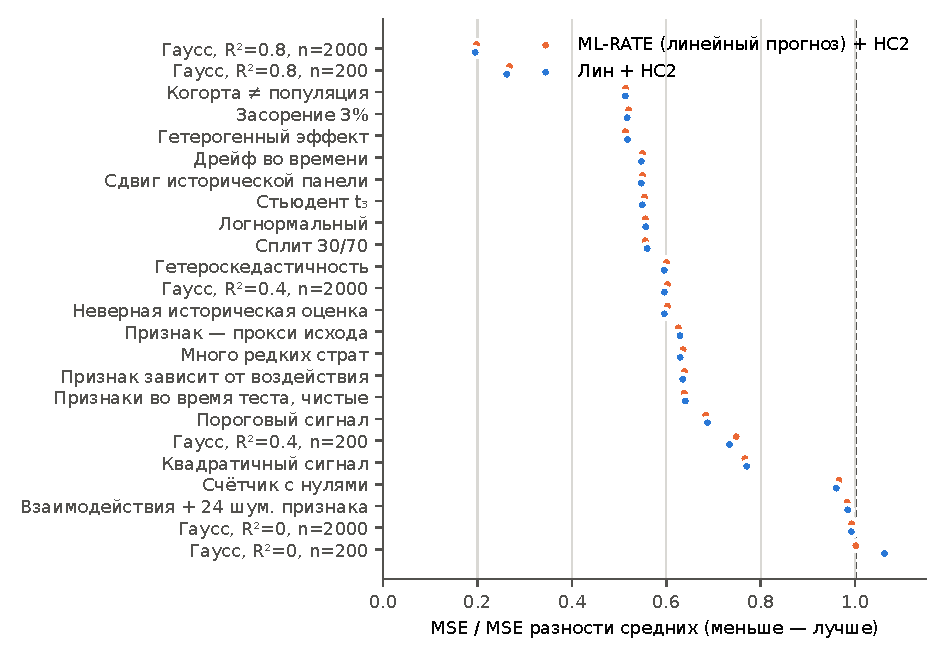
\includegraphics[width=0.9\textwidth]{figures/allworlds_mse.pdf}
\caption{MSE оценки эффекта относительно разности средних по мирам VarWar v3 (screening, $R=200$).
Пунктир --- уровень разности средних.}\label{fig:allworlds}
\end{figure}

\subsection{Независимые проверки теоретических утверждений}

Самодостаточный скрипт \code{docs/reports/lin\_hc2/sim\_theory.py} (numpy, 4000 реализаций на сценарий)
проверяет следующее.
\begin{itemize}
  \item \emph{Тождества}: $|\hat\tau_L-\text{закрытая форма}|=1.8\cdot10^{-15}$;
        $|\SE_{\text{HC2},K=0}-\SE_{\text{Welch}}|=3\cdot10^{-17}$.
  \item \emph{Кейс Фридмана} (табл.~\ref{tab:freedman}, рис.~\ref{fig:freedman}):
        $Y(0)=x+\varepsilon_0$, $Y(1)=\varepsilon_1$, $n=400$.
  \item \emph{Малые выборки} (рис.~\ref{fig:smalln}).
\end{itemize}

\begin{table}[h]
\centering\small
\caption{Кейс Фридмана: дисперсия относительно разности средних и покрытие 95\% CI.}\label{tab:freedman}
\footnotesize\setlength{\tabcolsep}{3.5pt}
\begin{tabular}{@{}lccc|ccc@{}}
\toprule
& \multicolumn{3}{c|}{$p=0.2$} & \multicolumn{3}{c}{$p=0.5$} \\
Метод & Var/Var$_{\text{DM}}$ & Покр. SATE & Покр. PATE & Var/Var$_{\text{DM}}$ & Покр. SATE & Покр. PATE \\
\midrule
Разность средних (Welch) & 1.00 & 0.989 & 0.953 & 1.00 & 0.995 & 0.954 \\
CUPED, общий $\theta$ & 1.40 & 0.983 & 0.953 & 0.68 & 0.999 & 0.951 \\
ANCOVA + HC2 & 1.42 & 0.982 & 0.951 & 0.68 & 0.999 & 0.951 \\
Лин + HC2 & \textbf{0.95} & 0.983 & 0.931 & 0.68 & 0.996 & 0.920 \\
Лин + HC2 + поправка \eqref{eq:pate} & 0.95 & 0.989 & \textbf{0.953} & 0.68 & 0.999 & \textbf{0.951} \\
\bottomrule
\end{tabular}
\end{table}

\begin{figure}[h]
\centering
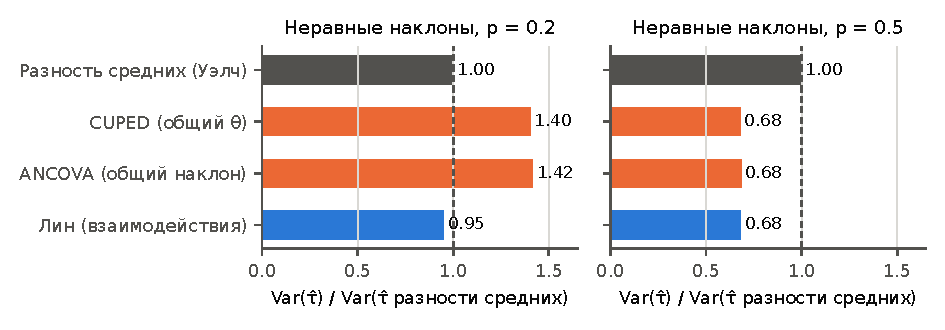
\includegraphics[width=0.95\textwidth]{figures/freedman.pdf}
\caption{При неравном сплите и разных наклонах оценки с общим коэффициентом
проигрывают даже разности средних; Лин --- нет. При $p=0.5$ все корректировки совпадают.}\label{fig:freedman}
\end{figure}

\begin{figure}[h]
\centering
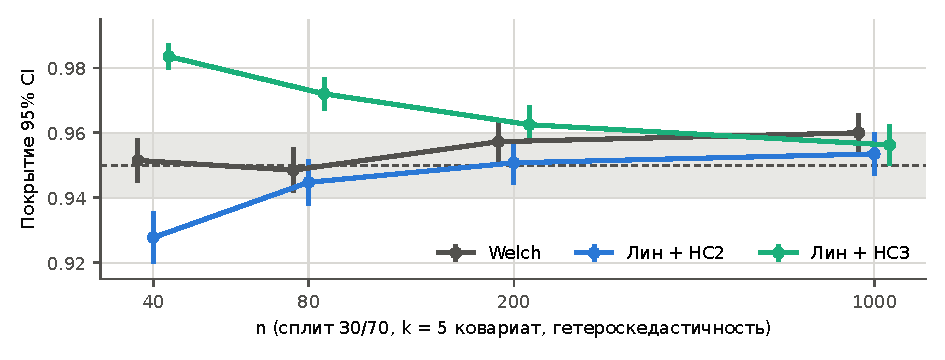
\includegraphics[width=0.95\textwidth]{figures/small_n.pdf}
\caption{Покрытие 95\% CI при малых выборках (полосы --- $\pm1.96$ MC-ошибки, серая зона --- $0.95\pm0.01$).}\label{fig:smalln}
\end{figure}

Высокое покрытие SATE в кейсе Фридмана (0.98--0.99) --- проявление
консервативности \eqref{eq:conservative}: эффект здесь сильно гетерогенен
($\tau_i=-x_i+\varepsilon_{1i}-\varepsilon_{0i}$), и дизайновая дисперсия заметно меньше
оцениваемой. Для PATE та же SE уже не консервативна, и нужна поправка.

%=====================================================================
\section{Когда метод проигрывает и как его применять}
%=====================================================================

\paragraph{Слабые места.}
\begin{enumerate}
  \item \textbf{Много ковариат при малом $n$ и слабом сигнале.} Каждая ковариата
        стоит двух параметров; при $R^2\approx0$ и $n=200$ MSE на 6\% выше, чем у разности средних.
  \item \textbf{Нелинейный сигнал.} Линейная проекция теряет часть $R^2$
        (в мирах с квадратичным и пороговым сигналом снижение MSE 23--31\% против $\approx40\%$ в линейном мире того же $R^2$).
        Лекарство --- прогноз ML как ковариата (раздел~5), сравнение запланировано в пересчёте.
  \item \textbf{Тяжёлые хвосты и выбросы.} OLS неробастна, хотя вывод остаётся
        валидным. Винзоризация исхода меняет estimand и должна фиксироваться заранее
        по предпериоду; преобразовывать ковариаты можно свободно.
  \item \textbf{PATE и сдвиг популяции.} Без поправки \eqref{eq:pate} интервал антиконсервативен.
  \item \textbf{Иные дизайны} (стратификация, рерандомизация). Лин остаётся валидным,
        но HC2 становится консервативной, а выигрыш над уже сбалансированным
        дизайном мал. Корректный вывод для рерандомизации требует отдельных формул.
\end{enumerate}

\paragraph{Чек-лист применения.}
\begin{itemize}
  \item Единица анализа совпадает с единицей рандомизации.
  \item Ковариаты строго до воздействия; список фиксируется до эксперимента.
        Лаг самой метрики --- в первую очередь.
  \item $K\ll n_{\min}$; категориальные признаки --- дамми без референсного уровня; проверка ранга.
  \item Центрирование по всей анализируемой выборке; регрессия с взаимодействиями.
  \item SE: HC2 (HC3 при малых $n$); квантиль $t_\nu$; для PATE --- поправка \eqref{eq:pate}.
  \item Если используется ML-прогноз --- только предпериод или cross-fitting, без $T$ в модели.
  \item Отчёт: оценка, CI, p-value, снижение дисперсии $1-\hat V_L/\hat V_{\text{DM}}$,
        баланс ковариат как диагностика (но не как условие анализа).
\end{itemize}

%=====================================================================
\section{Ограничения доказательной базы и пересчёт}
%=====================================================================

Сильные доказательства валидности и выигрыша Лина получены пока для одного
подтверждающего мира ($R=1000$); по остальным мирам доступен screening с $R=200$ и
коррелированными seed. Конкуренты с преобразованием метрики (CUPED, CUPAC) в v3
оценивались с неверной SE, поэтому их сравнение с Лином по валидности ещё не проведено.
В ветке \code{rerun/v3.1} исправлены ошибки стенда и добавлены миры, где методы
различаются по теории (неравный сплит с гетерогенностью, панельная метрика, нелинейный
сигнал). Подготовлен пересчёт: screening по всем мирам ($R=500$) и confirmation
финалистов ($R=2000$). Таблицы \ref{tab:confirm} и рис.~\ref{fig:allworlds}
будут заменены по его итогам.

\begin{thebibliography}{99}
\bibitem[Lin(2013)]{lin2013} W.~Lin. Agnostic notes on regression adjustments to experimental data:
  Reexamining Freedman's critique. \emph{The Annals of Applied Statistics}, 7(1):295--318, 2013.
\bibitem[Freedman(2008)]{freedman2008} D.~A.~Freedman. On regression adjustments to experimental data.
  \emph{Advances in Applied Mathematics}, 40(2):180--193, 2008.
\bibitem[Li and Ding(2017)]{lidingclt2017} X.~Li, P.~Ding. General forms of finite population central limit
  theorems with applications to causal inference. \emph{JASA}, 112(520):1759--1769, 2017.
\bibitem[Neyman(1923)]{neyman1923} J.~Neyman. On the application of probability theory to agricultural
  experiments (1923; transl. \emph{Statistical Science}, 5(4):465--472, 1990).
\bibitem[White(1980)]{whitehc} H.~White. A heteroskedasticity-consistent covariance matrix estimator and a
  direct test for heteroskedasticity. \emph{Econometrica}, 48(4):817--838, 1980.
\bibitem[MacKinnon and White(1985)]{mackinnonwhite1985} J.~G.~MacKinnon, H.~White. Some
  heteroskedasticity-consistent covariance matrix estimators with improved finite sample properties.
  \emph{Journal of Econometrics}, 29(3):305--325, 1985.
\bibitem[Bell and McCaffrey(2002)]{bellmccaffrey2002} R.~M.~Bell, D.~F.~McCaffrey. Bias reduction in standard
  errors for linear regression with multi-stage samples. \emph{Survey Methodology}, 28(2):169--181, 2002.
\bibitem[Imbens and Kolesár(2016)]{imbenskolesar2016} G.~W.~Imbens, M.~Kolesár. Robust standard errors in small
  samples: Some practical advice. \emph{Review of Economics and Statistics}, 98(4):701--712, 2016.
\bibitem[Deng et~al.(2013)]{deng2013cuped} A.~Deng, Y.~Xu, R.~Kohavi, T.~Walker. Improving the sensitivity of
  online controlled experiments by utilizing pre-experiment data. \emph{WSDM}, 2013.
\bibitem[Guo et~al.(2021)]{guo2021mlrate} Y.~Guo, D.~Coey, M.~Konutgan, W.~Li, C.~Schoener, M.~Goldman. Machine
  learning for variance reduction in online experiments. \emph{NeurIPS}, 2021.
\bibitem[Chernozhukov et~al.(2018)]{chernozhukov2018dml} V.~Chernozhukov et~al. Double/debiased machine learning
  for treatment and structural parameters. \emph{The Econometrics Journal}, 21(1):C1--C68, 2018.
\bibitem[Negi and Wooldridge(2021)]{negiwooldridge2021} A.~Negi, J.~M.~Wooldridge. Revisiting regression
  adjustment in experiments with heterogeneous treatment effects. \emph{Econometric Reviews}, 40(5):504--534, 2021.
\bibitem[Imbens and Rubin(2015)]{imbensrubin2015} G.~W.~Imbens, D.~B.~Rubin. \emph{Causal Inference for
  Statistics, Social, and Biomedical Sciences}. Cambridge University Press, 2015.
\end{thebibliography}

\appendix
\section{Вывод оптимального коэффициента}
Для фиксированного $\theta$ разложим $\hat\tau(\theta)=\overline{(Y-\theta\T X)}_1-\overline{(Y-\theta\T X)}_0$ ---
разность средних «скорректированного» исхода $Y_i(t)-\theta\T X_i$. По теореме Неймана
\citep{neyman1923, imbensrubin2015}
$n\Var\hat\tau(\theta)=S^2_1(\theta)/p+S^2_0(\theta)/(1-p)-S^2_\tau$, где
$S^2_t(\theta)=S^2_{Y(t)}-2\theta\T S_{XY(t)}+\theta\T S_{XX}\theta$.
Условие первого порядка:
$-2S_{XY(1)}/p-2S_{XY(0)}/(1-p)+2\bigl(1/p+1/(1-p)\bigr)S_{XX}\theta=0$, откуда
$\theta^*=(1-p)\beta_1+p\beta_0$ с $\beta_t=S_{XX}^{-1}S_{XY(t)}$. Подстановка
$\theta_{\text{pool}}=p\beta_1+(1-p)\beta_0$ даёт разность
$(\theta_{\text{pool}}-\theta^*)\T S_{XX}(\theta_{\text{pool}}-\theta^*)\bigl(1/p+1/(1-p)\bigr)$
$=(1-2p)^2(\beta_1-\beta_0)\T S_{XX}(\beta_1-\beta_0)/(p(1-p))$, то есть \eqref{eq:freedman-loss}.
\end{document}
